\documentclass[a4paper]{scrartcl}

% \usepackage{amsmath}
\usepackage[english]{babel}
% \usepackage{lmodern}
\usepackage{anyfontsize}
\usepackage{listings}
\usepackage{amssymb}% http://ctan.org/pkg/amssymb
\usepackage{pifont}% http://ctan.org/pkg/pifont
\newcommand{\cmark}{\ding{51}}%
\newcommand{\xmark}{\ding{55}}%
\usepackage{color}
\usepackage{xcolor}
\usepackage{svg}
\usepackage{graphicx}

\definecolor{mygreen}{rgb}{0,0.6,0}
\definecolor{mygray}{rgb}{0.5,0.5,0.5}
\definecolor{mymauve}{rgb}{0.58,0,0.82}
\definecolor{mainblue}{HTML}{2F88BD}%{009EFC}
\newcommand{\blu}[1]{\textcolor{mainblue}{#1}}

\lstset{ %
  backgroundcolor=\color{white},   % choose the background color; you must add \usepackage{color} or \usepackage{xcolor}; should come as last argument
  basicstyle=\footnotesize,        % the size of the fonts that are used for the code
  breakatwhitespace=false,         % sets if automatic breaks should only happen at whitespace
  breaklines=true,                 % sets automatic line breaking
  captionpos=b,                    % sets the caption-position to bottom
  commentstyle=\color{mygreen},    % comment style
  % deletekeywords={...},            % if you want to delete keywords from the given language
  escapeinside={\%*}{*)},          % if you want to add LaTeX within your code
  extendedchars=true,              % lets you use non-ASCII characters; for 8-bits encodings only, does not work with UTF-8
  frame=single,	                   % adds a frame around the code
  keepspaces=true,                 % keeps spaces in text, useful for keeping indentation of code (possibly needs columns=flexible)
  keywordstyle=\color{blue},       % keyword style
  language=Python,                 % the language of the code
  morekeywords={*,...},            % if you want to add more keywords to the set
  % numbers=left,                    % where to put the line-numbers; possible values are (none, left, right)
  % numbersep=5pt,                   % how far the line-numbers are from the code
  % numberstyle=\tiny\color{mygray}, % the style that is used for the line-numbers
  rulecolor=\color{black},         % if not set, the frame-color may be changed on line-breaks within not-black text (e.g. comments (green here))
  showspaces=false,                % show spaces everywhere adding particular underscores; it overrides 'showstringspaces'
  showstringspaces=false,          % underline spaces within strings only
  % showtabs=true,                  % show tabs within strings adding particular underscores
  % stepnumber=2,                    % the step between two line-numbers. If it's 1, each line will be numbered
  stringstyle=\color{mymauve},     % string literal style
  tabsize=4,	                   % sets default tabsize to 2 spaces
  title=\lstname                   % show the filename of files included with \lstinputlisting; also try caption instead of title
}

\begin{document}
\section{Inverted Index}
\paragraph{Idea:} For each word, pre-compute and store a \emph{sorted} list of
ids of documents containing them.

$\Rightarrow$ Inverted Lists:
\begin{table}[!htbp]n
  \centering
  \caption{Example of inverted lists}
  \label{tab:inverted_list}
  \begin{tabular}{ll}
  astronauts& 13, 57, 64, 77, 104, ... \\
  moon & 5, 23, 57, 63, 104, 257, ...
  \end{tabular}
\end{table}

\lstinputlisting[caption=Intersecting sorted lists in linear
time]{code/intersect.py}
\paragraph{Querying with more than 2 keywords:}
\begin{enumerate}
\item Intersect $L_1$ and $L_2\rightarrow L_{12}$
\item Intersect $L_{12}$ and $L_3\rightarrow L_{123}$
\item ...
\end{enumerate}
Possible Optimizations:
\begin{itemize}
\item Order the lists s.t. $|L_1|\le|L_2|\le|L_3|\le...\le|L_k|$
\end{itemize}

\section{Ranking}
Ways to rank the relevance of the found entries with respect to the query.
\begin{itemize}
\item In the inverted lists, each doc id also has a \emph{score}
  \begin{table}[!htbp]
    \centering
    \caption{Scoring}
    \label{tab:scored_list}
    \begin{tabular}{ll}
      astronauts& 13:0.2, 57:0.5, 64:0.3, 77:0.25, 104:0.1, ... \\
      moon & 5:0.3, 23:0.6, 57:0.8, 63:0.2, 104:0.1, 257:0.9, ...
    \end{tabular}
  \end{table}
\item When merging, aggregate the scores and then sort.
\item Doc ID and score (or more info): \emph{posting}
\item Sorting only the top-$k$ hits takes $\Theta(n)$ time for constant $k$.
  (with heapsort)
\end{itemize}

\subsection{Scoring algorithms}
\label{sec:scoring_algorithms}
\begin{itemize}
\item \emph{Term frequency} (tf): Number of times a word occurs in a document
  \begin{itemize}
  \item Problem: Words like of, a, and, the,...
  \item Just ignore these
  \end{itemize}
\item \emph{Inverse document frequency} (idf):
  \begin{equation}
    \mathrm{idf}=\log_2\frac{N}{\mathrm{df}}
  \end{equation}
  $N$: Total number of documents, $\mathrm{df}$: Document frequency (number of
  documents containing a particular word)
\item Combining tf and idf: good way to decrease the influence of “of”, “the”,
  “and”, ...

  Problems with tf.idf:
  \begin{itemize}
  \item \textbf{Problem 1:} Longer documents are automatically weighted higher.
  \item \textbf{Problem 2:} Double tf doesn't mean it's doubly “about“ the query.
  \end{itemize}
\item \emph{BM25}
  \begin{equation}
    \mathrm{BM25}=\mathrm{tf}^*\cdot \log_2\frac{N}{\mathrm{df}}
  \end{equation}
  \begin{equation}
    \mathrm{tf}^*=\mathrm{tf}\cdot \frac{(k+1)}{k\cdot(1-b + b \cdot \frac{\mathrm{DL}}{\mathrm{AVDL}})}
  \end{equation}
  DL: Document length, AVDL: average document length. $k,b$: Magic numbers (good
  setting: $k=1.75, b=0.75$)
  \begin{itemize}
  \item Normal tf.idf: $k=\infty, b=0$
  \end{itemize}
\end{itemize}

\subsection{Evaluation}
\subsubsection{Precision}
\begin{itemize}
\item Precision (\emph{P@k}): Percentage of relevant documents among the top $k$
  \begin{itemize}
  \item Example:\\
    \begin{tabular}{ll}
      Query:& matrix movies \\
      Relevant:& 10, 582, 877, 10003 \\
      Result list:& 582(\cmark), 17(\xmark), 5777(\xmark), 10003(\cmark), 10(\cmark), 37(\xmark),...\\
      \emph{P@1}:&100\% \\
      \emph{P@2}:&50\% \\
      \emph{P@3}:&33\% \\
      \emph{P@4}:&50\% \\
      \emph{P@5}:&60\% \\
    \end{tabular}
  \end{itemize}
\item \emph{P@R}: \emph{P@k}, where $k=$amount of relevant documents
\item \emph{Average Precision} (AP)
  \begin{itemize}
  \item $R_1,R_2,...,R_k$: Sorted list of positions of the relevant documents in
    the result list. \\
    \begin{tabular}{ll}
      Query:& matrix movies \\
      Relevant:& 10, 582, 877, 10003 \\
      Result list:& 582(\cmark), 17(\xmark), 5777(\xmark), 10003(\cmark), 10(\cmark), 37(\xmark),...,877(\cmark) \\
      $R_1,...,R_4$:& 1,4,5,40 \\
      $P@R_1$,...,$P@R_4$:& 100\%, 50\%, 60\%, 10\% \\
      AP:& (100\% + 50\%, 60\%, 10\%)/4 = 55\%
    \end{tabular}
  \end{itemize}
\end{itemize}

\subsubsection{Mean precisions}
Measure quality of a system by taking the mean of a given measure over all
queries:
\begin{itemize}
\item \emph{MP@k}: mean of the P@k values over all queries
\item \emph{MP@R}: mean of the P@R values over all queries
\item \emph{MAP}: mean of the AP values over all queries
\end{itemize}

\subsubsection{Discounted cumulative gain (DCG, nDCG)}
Relevance not binary (i.e.: 0: not relevant, 1: somewhat relevant, 2: very
relevant)
\begin{itemize}
\item \emph{Cumulative gain:} \[CG@k=\sum_{i=1,...,k} \mathrm{rel}_i\]
\item \emph{Discounted CG:} \[DCG@k = \mathrm{rel}_i +
  \sum_{i=2,...,k}\frac{\mathrm{rel}_i}{\log_2 i}\]
\item Normalize by maximally achievable value:
\item \emph{Ideal DCG}: \[iDCG@k=DCG@k\ \mathrm{of\ ideal\ ranking}\]
\item \emph{Normalized DCG}: \[nDCG@k = \frac{DCG@k}{iDCG@k}\]
\end{itemize}

\subsubsection{Binary preference (bpref)}
If you have way more unjudged documents than judged ones
\[\mathrm{bpref}=\frac{1}{|R|}\cdot\sum_{r\in RR}\frac{1-|NR(r)|}{\min(|R|,|N|)}\]
\begin{itemize}
\item $R$: Set of all judged relevant docs
\item $N$: Set of all judged not relevant docs
\item $RR:$ Docs in $R$ and in result list
\item $NR(r\in RR):$ docs from the $|R|$ top-ranked from $N$ ranked before $r$
\item Example: Result list with 7 judged documents overall\\ 
    \begin{tabular}{ll|}
      \#1&judged relevant\\
      \#2&not judged\\
      \#3&not judged\\
      \#4&judged not relevant\\
      \#5&judged relevant\\
    \end{tabular}
    Not in result list:
    \begin{tabular}{l}
      $A$, judged relevant \\
      $X, Y, Z$, judged not relevant
    \end{tabular}
    \begin{itemize}
    \item $R=\{\#1, \#5, A\} $
    \item $N=\{\#4, X, Y, Z\}$
    \item $RR=\{\#1,\#5\}$
    \item $NR(\#1)= \{\}, |NR(\#1)|=0$
    \item $NR(\#5)= \{\#4\}, |NR(\#5)|=1$
\[\Rightarrow\mathrm{bpref} = \frac{1}{3}\left( \left( 1-\frac{0}{3} \right) +
        \left( 1-\frac{1}{3} \right) \right) = \frac{5}{9}\]
    \end{itemize}
\end{itemize}

\section{Efficiency tuning}

\subsection{Non-algorithmic improvements}
\begin{itemize}
\item Instead of lists: Native arrays
\item Increase predictability by reducing conditional parts of code
  \begin{itemize}
  \item Pipelining: Improve predictability by evaluate to the same boolean value
    most of the time.
  \item Sentinels: Special elements to avoid testing for index out of bound
  \end{itemize}
\end{itemize}

\subsection{Algorithmic improvements}
\begin{itemize}
\item Binary search in the longer list (Complexity $\Theta(k\cdot \log n)$)\\
  Good for small $k$, but for $k=\Theta(n)$, this is $\Theta(n\log
  n)\Rightarrow$ slower than zipper.
\item Binary search in remainder of longer list
  \begin{itemize}
  \item Time complexity in the best case: $\Theta(k+\log n)$ (First element from
    A towards the end of list B)
  \item Time complexity in the worst case: $\Theta(k\cdot \log n)$ (All elements
    of A at the beginning of list B)
  \item Typical time complexity: $\Theta(k\cdot \log n)$ (Elements of A evenly
    distributed over list B)
  \end{itemize}
\item Galloping search: Exponential search to get an upper bound, then binary
  search
  \[\mathcal{O}\left(k\cdot \log\left(1+\frac{n}{k}\right)\right)\]
  Note: Always $\mathcal{O}(n)\Rightarrow$ at least as good as Zipper!
  (\emph{asymptotically optimal})
\item Skip pointers: heuristically skip elements of the longer list.
\end{itemize}

\section{Compression}
Gap encoding: Store differences from one item to the next (of a sorted list)

\subsection{Elias-Gamma}

\begin{itemize}
\item Write $ \left\lfloor
    \log_2 x
  \right\rfloor$ zeros, then $x$ in binary
\item Prefix-free
\item Length for $x$: $2\cdot\lfloor \log_2 x \rfloor + 1$ bits
\end{itemize}
\begin{table}[!htbp]
  \centering
  \begin{tabular}{ll}
    1&1\\
    2&010\\
    3&011\\
    4&00100\\
    \multicolumn{2}{c}{...}\\
    10&0001010
  \end{tabular}
  \caption{Elias-Gamma}
  \label{tab:elias_gamma}
\end{table}
\subsection{Elias-Delta}
\begin{itemize}
\item Write $\lfloor {\log_2 x} \rfloor \blu{+ 1}$ in Elias-Gamma, followed by $x$ in
  binary, but \textcolor{mainblue}{\textbf{without the leading 1!}}
\item Prefix-free
\item Lenght for $x$: $\lfloor {\log_2 x} + 2\log_2\log_2 x + \mathcal{O}(1) \rfloor$
\end{itemize}
\begin{table}[!htbp]
  \centering
  \begin{tabular}{ll}
    1&1\\
    2&010\blu{0}\\
    3&010\blu{1}\\
    4&011\blu{00}\\
    5&011\blu{01}\\
    6&011\blu{10}\\
    \multicolumn{2}{c}{...}\\
    10&00100\blu{010}
  \end{tabular}
  \caption{Elias-Delta}
  \label{tab:elias_delta}
\end{table}
\subsection{Golomb}
\label{sec:golomb}
\begin{itemize}
\item Code-length:
  \[L_x = \left\lfloor \frac{x}{M} \right\rfloor + 1 +
  \left\lceil \log_2 M \right\rceil\]
\item Comes with an integer parameter $M$ (``modulus'')
\item Write $x$ as $q\cdot M + r$
  \begin{itemize}
  \item $q = x \div M$
  \item $r = x\ \mathrm{mod}\ M$
  \end{itemize}
\item Code for $x$:
  \begin{itemize}
  \item $q$ written in unary with 0s ($\left\lfloor {\frac{x}{M}} \right\rfloor$
    bits)
  \item single 1 as delimiter (1 bit)
  \item $r$ written in binary ($\left\lceil {\log_2 M} \right\rceil$ bits)
  \end{itemize}
\item Example:
  \[M=16, x=42\]
  \[q = 42\div 16 = 2 = 00\ \mathrm{(in\ unary)}\]
  \[r = 42\ \mathrm{mod}\ 16 = 10 = 1010\ \mathrm{(in\ binary)}\]
  \[\Rightarrow \mathrm{Golomb\ code:}\ 0011010\]
\end{itemize}
\subsection{Variable-Byte}
\label{sec:variable_byte}

\begin{itemize}
\item Gets rid of the bit fiddling
\end{itemize}

\subsubsection{Example: UTF-8}
\label{sec:utf-8}
\begin{itemize}
\item Start a number with the total amount of bytes the whole number needs
  written in unary 1's
\item Insert a delimiter 0 and write the number you want
\item For every continuation byte, start it with a 10-prefix
\end{itemize}

\section{Entropy}
\label{sec:entropy}
Definition of entropy of a discrete random variable $X$
\[H(X) = -\sum_i p_i \log_2 p_i\]

\subsection{Entropy-optimal codes}
\label{sec:entropy_optimal_codes}
A code is optimal for distribution $p_i$ if:
\[L_i\le 1 - \log_2 p_i\]
\subsection{Shannon's source coding theorem}
\label{sec:shannon_theorem}

\begin{itemize}
\item Let $X$ be a random variable with \blu{finite range}
\item For an arbitrary prefix-free (PF) encoding, let $L_i$ be the length of the
  code for $i \in \mathrm{range}(X)$
\item[$\Rightarrow$] For any PF encoding it holds: $\mathbb{E}\{L_X\}\ge H(X)$
\item[$\Rightarrow$] There is a PF encoding with: $\mathbb{E}\{L_X\}\le H(X) + 1$
\item In words:\\
  \blu{No code can be better than the entropy and there is always a code that's
    (almost) as good!}
\item Kraft inequality ($L_i$ is the length of a code):
\[\sum_{i\in X}^X 2^{-L_i}\le 1\]
\end{itemize}

\subsection{Huffman coding}
\label{sec:huffman_coding}
\begin{itemize}
\item Has $2^{\max L_i}$ leaves.
\item Encoding:
  \begin{itemize}
  \item Sort symbols to encode by frequency
  \item Start with least frequent symbols, and write their frequency next to
    them.
  \item Bundle words with the same frequency together and connect them with a
    node containing their combined frequencies.
  \item This combined frequency gets bundled with symbols with the same
    frequency as the combined one.
  \item Continue until you reach a root node.
  \item Denote right edges with 1, left with 0.
  \end{itemize}
\item Decoding:
  \begin{itemize}
  \item Start at the root node
  \item For every 1 go right, for every 0 go left...
  \item ... until you hit a symbol
  \end{itemize}
\end{itemize}
\begin{figure}[!htbp]
  \centering
  \includesvg[width=0.8\textwidth]{figures/huffman_tree}
  \caption{Huffman tree}
  \label{fig:huffman_tree}
\end{figure}

\section{Fuzzy Search}
\label{sec:fuzzy_search}

\subsection{Edit distance}
\label{sec:edit_distance}
If the characters aren't equal, take the minimum of left, up and
left-up-diagonal + 1. If the characters are equal, take the diagonal and don't
add 1.
\begin{figure}[!htbp]
  \centering
  % 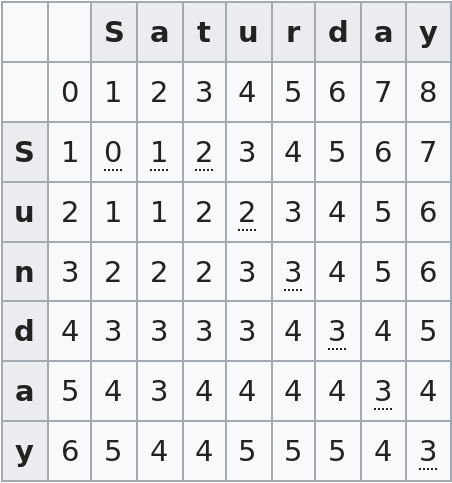
\includegraphics[height=60mm]{figures/edit_distance}
  % TODO: add the edit distance figure
  foo
  \caption{Edit distance table}
  \label{fig:edit_distance}
\end{figure}

\subsection{Prefix edit distance (PED)}
\label{sec:prefix_edit_distance}
\[\mathrm{PED}(x,y)=\min \mathrm{ED}(x,y'),\ \mathrm{where\ }y'\mathrm{\ is\ a\ prefix\ of\ }y\]
\begin{itemize}
\item Example:
  \[\mathrm{PED}(\mathrm{uni}, \mathrm{\blu{uni}versity}) = 0\ (\mathrm{ED}=7)\]
  \[\mathrm{PED}(\mathrm{uniwer}, \mathrm{\blu{univer}sity}) = 1\ (\mathrm{ED}=5)\]
\item Computation:
  \begin{itemize}
  \item create $|x|\cdot|y|$-table
  \item PED is the minimum of the entries in the last row
  \item when $|x|<<|y|$ and only $\mathrm{PED}(x,y)\le\delta$ is important, then
    only compute the first $|x|+\delta+1$ columns
  \end{itemize}

\end{itemize}

\subsection{q-Gram Index}
\label{sec:q_gram_index}
\begin{itemize}
\item $q$-gram: all substrings of length $q$
\item number of $q$-grams: $|x|-q+1$
\item size with padding: $|x|+q-1$
\item $q$-gram index: inverted list of the strings (from the input set), sorted
  lexicographically.
\item Space consumption: Each record contributes $|x|+Q$ ids to the inverted
  lists. $Q$ is the total number of padding characters (for one-sided padding:
  $Q=2$)
\end{itemize}
\subsection{Fuzzy search algorithm}
\label{sec:fuzzy_search_algorithm}
\begin{itemize}
\item Let's say, we only look at $x$ and $y$ with $ED(x,y)=\delta$
\item With $x'$ and $y'$ being padded versions of $x$ and $y$, the amount of
  $q$-grams they have in common is:
  \begin{equation}
  \mathrm{comm}(x',y')\le \max(|x|,|y|)-1-(\delta - 1)\cdot q\label{eq:least_common_qgram}
\end{equation}

\item Processing a query
  \begin{enumerate}
  \item Pad $x$
  \item compute the $q$-grams of $x$
  \item fetch and merge all ids of every $q$-gram, counting how often each id
    shows up in the merge
  \item for each entry, you compute the amount minimum in common number
    \begin{enumerate}
    \item If it's too low, according to (\ref{eq:least_common_qgram}), discard
      it.
    \item If not: Compute the edit-distance
    \end{enumerate}
    \lstinputlisting[caption=Processing a query]{code/fuzzy_search.py}
  \end{enumerate}
\item Changes when using the Prefix-edit-Distance (PED): The least common amount
  (\ref{eq:least_common_qgram}) reduces to:
  \begin{equation}
    \label{eq:least_common_ped}
    \mathrm{comm}(x',y')\ge |x|-q\cdot \delta
  \end{equation}
\end{itemize}

% \section{Web applications}
% TODO: Lecture 6, 7 (ausdrucken?)

\section{Vector-Space Model}
\label{sec:vector_space_model}
\begin{itemize}
\item The big idea: Just represent the inverted index as a term-document matrix
  (words are called terms now):
  \begin{table}[h!tbp]
    \centering
    \begin{tabular}{lcccccc}
      &$D_1$&$D_2$&$D_3$&$D_4$&$D_5$&$D_6$ \\
      internet & 1 & 1 & 0& 1 & 0 & 0 \\
      web & 1 & 0 & 1 & 1 & 0 & 0\\
      surfing & 1 & 1 & 1 & 2 & 1 & 1 \\
      beach & 0 & 0 & 0 & 1 & 1 & 1\\
    \end{tabular}
    \caption{Term-Document matrix}
    \label{tab:term_document_matrix}
  \end{table}
\item Queries are represented as a vector
\item Results: ($q$: query, $A$: Term-document-matrix)
  \begin{equation}
    \label{eq:vsm_result}
     r = q^\top \cdot A
  \end{equation}
\end{itemize}

\subsection{Sparse matrices}
\label{sec:sparse_matrices}
\begin{itemize}
\item Sparse matrices only store the non-zero entries.
\item row-major: Store row index first
\item column-major: Store col index first
\item Note: sparse row-major representation of a document matrix is basically
  its' \blu{inverted index}.
  \begin{figure}[h!tbp]
    \centering
    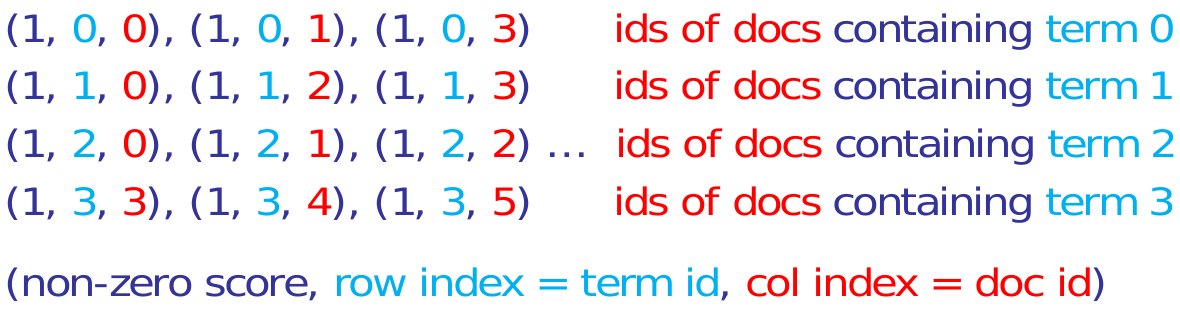
\includegraphics[width=0.8\textwidth]{figures/sparse_ii}
    \caption{Sparse row-major representation of an inverted index}
    \label{fig:sparse_ii}
  \end{figure}
\item idf can be seen as a normalization (multiply each row by a certain factor,
  i.e. the idf), it's not the same thing, though!
\end{itemize}

% \section{Clustering/K-means}
% \label{sec:clustering_k_means}
% TODO: print out lecture 9?

\section{Useful stuff}

\subsection{Lagrange optimization}
Function to minimize $f(x)$, constraints $g(x)\ge 0$. Lagrange function:
\[\mathcal{L}(x,\lambda)=f(x)-\lambda g(x)\]
Set
\[\frac{\mathrm{d}}{\mathrm{d}x}\mathcal{L}=0\] and
\[\frac{\mathrm{d}}{\mathrm{d}\lambda}\mathcal{L}=0\]

% Stuff to print:
% - Solution to sheet 4

\end{document}

%%% Local Variables:
%%% coding: utf-8
%%% mode: latex
%%% TeX-engine: xetex
%%% TeX-master: t
%%% End:
